\documentclass{beamer}
\usepackage{booktabs}
\usepackage{pdfpages}
\usepackage{mathtools}
\usepackage{enumerate}
\usepackage{enumitem}
\usepackage{multirow,tabularx}
\usepackage{booktabs}
\usepackage{pdfpages}
\usepackage{proof}
\usepackage{cancel}
\usepackage{chronology}
\usepackage{graphicx}
\usepackage{ulem}
\usepackage{amsmath}
\usepackage{amssymb}
\usepackage{color}

\PassOptionsToPackage{usenames,dvipsnames,svgnames}{xcolor}  
\usepackage{tikz}
\usepackage{tkz-graph}
\usetikzlibrary[positioning,arrows,automata]
\usepackage{wasysym}
\usepackage{proof}
\usepackage{cancel}
\usepackage{chronology}
\usepackage{graphicx}
\usepackage{ulem}
\usepackage{amsmath}
\usepackage{amssymb}
\usepackage{color}
\usepackage{xcolor}
\usepackage{soul}
%\usepackage{pstricks}
%\setbeamertemplate{navigation symbols}{}

\newcommand{\myul}[2][blue]{\sethlcolor{#1}\hl{#2}\setulcolor{black}}

\newcommand<>{\cunderline}[3]{\only<#1>{#3}\only<#2>{\underline{#3}}}
\newcommand<>{\cem}[3]{\only<#1>{#3}\only<#2>{\ul{#3}}}
\newcommand<>{\cgray}[3]{\only<#1>{#3}\only<#2>{\textcolor{gray}{#3}}}
\newcommand<>{\colorize}[4]{\only<#1>{#4}\only<#2>{\textcolor{#3}{#4}}}

\addtobeamertemplate{navigation symbols}{}{%
    \usebeamerfont{footline}%
    \usebeamercolor[fg]{footline}%
    \hspace{1em}%
    \insertframenumber/\inserttotalframenumber
}

\renewcommand{\em}{\itshape}

\mode<presentation>
% {
%   \usecolortheme{crane}
% %  \usetheme{Frankfurt}
% }
\mode<presentation>
{
  \usecolortheme{dove}
}


\title[Ontologies]{Part 2: Machine learning with ontologies}

\author{Robert Hoehndorf}

\date{}

\begin{document}

\begin{frame}
  \titlepage
\end{frame}

\section{Machine learning and ontologies}

\begin{frame}
  \frametitle{Challenges with semantic similarity}
  \begin{itemize}
  \item not data-driven but hand-crafted
  \item not task-specific
  \item usually outputs a single value
  \item hard to chose a similarity measure
  \item usually graph-based and losing some information
  \end{itemize}
  Next: machine learning methods for and with ontologies
\end{frame}

\begin{frame}
  \frametitle{Machine learning with ontologies: Overview}
  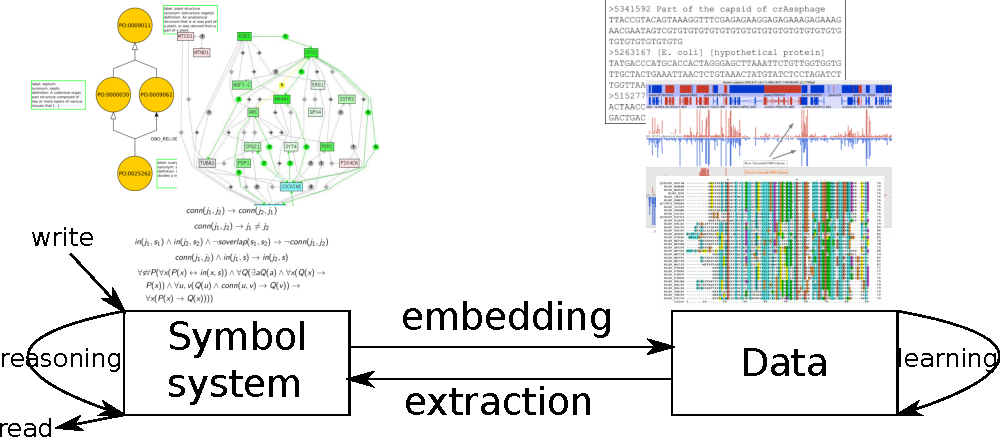
\includegraphics[width=\textwidth]{neuro-symbolic-cycle.pdf}
%  \pause
  \begin{columns}
    \begin{column}{.5\textwidth}
      \begin{itemize}[leftmargin=2cm]
      \item phenotype
      \item function
      \item disease
      \end{itemize}
    \end{column}
    \begin{column}{.5\textwidth}
      \begin{itemize}[leftmargin=2cm]
      \item genotype
      \item protein sequence
      \item expression
      \end{itemize}
    \end{column}
  \end{columns}
\end{frame}

\begin{frame}
  \frametitle{Embedding formal knowledge}
  \begin{block}{Embedding}
    An embedding is a map (morphism) from one mathematical structure
    $X$ into another structure $Y$:\\$f : X \xhookrightarrow{} Y$\\
    such that $X$ is preserved in $Y$.
  \end{block}
  \begin{itemize}
  \item $Y$ may be more suitable than $X$ for some operations/algorithms.
    \begin{itemize}
    \item similarity
    \item gradients, optimization
    \end{itemize}
  \end{itemize}
  \pause
  We want to embed {\em ontologies} in $\Re^n$. Approaches:
  \begin{itemize}
  \item graph-based
  \item syntactic
  \item model-theoretic
  \end{itemize}
\end{frame}

\begin{frame}
  \frametitle{Random walks}
  \begin{columns}
    \begin{column}{.6\textwidth}
      \resizebox{1\textwidth}{!}{%
        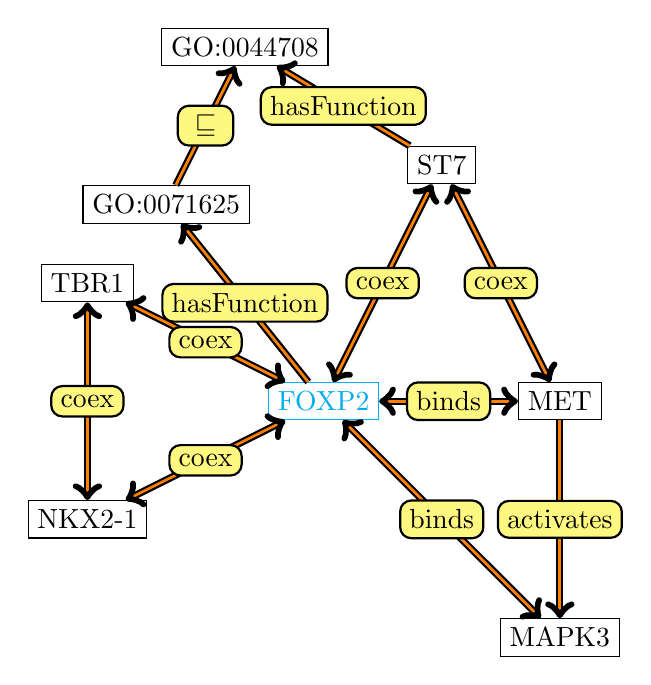
\begin{tikzpicture}
%          \SetUpEdge[lw = 1pt, color = black]
          \GraphInit[vstyle=Shade]
          \tikzset{
            LabelStyle/.style = { rectangle, rounded corners, draw,
              minimum width = 2em, fill = yellow!50,
              text = black },
            VertexStyle/.append style = { inner sep=5pt,
              font = \Large\bfseries},
            EdgeStyle/.append style = {->} }
          
          \SetGraphUnit{5}
          % \tikzset{VertexStyle/.append style={fill}}
          % \tikzset{EdgeStyle/.style={->}}
          \node[draw, color=cyan] (FOXP2) at (0,0) {FOXP2};
          \node[draw] (MET) at (3,0) {MET};
          \node[draw] (ST7) at (1.5,3) {ST7};
          \node[draw] (MAPK3) at (3,-3) {MAPK3};
          \node[draw] (GO0071625) at (-2,2.5) {GO:0071625};
          \node[draw] (GO0044708) at (-1,4.5) {GO:0044708};
          \node[draw] (TBR1) at (-3,1.5) {TBR1};
          \node[draw] (NKX2-1) at (-3,-1.5) {NKX2-1};
          \begin{scope}[/tikz/handle active characters in nodes=false]
          \Edge[label=activates](MET)(MAPK3)
          \Edge[label=hasFunction](FOXP2)(GO0071625)
          \Edge[label=hasFunction](ST7)(GO0044708)
          \Edge[label=$\sqsubseteq$](GO0071625)(GO0044708)

          \tikzset{EdgeStyle/.append style={<->}}
          \Edge[label=binds](FOXP2)(MET)
          \Edge[label=binds](FOXP2)(MAPK3)
          \Edge[label=coex](FOXP2)(TBR1)
          \Edge[label=coex](FOXP2)(NKX2-1)
          \Edge[label=coex](FOXP2)(ST7)
          \Edge[label=coex](MET)(ST7)
          \Edge[label=coex](NKX2-1)(TBR1)
          \end{scope}
          % \tikzset{EdgeStyle/.style={->}}
          % \Edge[label=hf](FOXP2)(GO0044708)
          % \draw[label=binds] (FOXP2) to (MET);
          % \Edge[label=binds](FOXP2)(MET)
          % \Edge[label=activates](MET)(MAPK3)
          % \Edge[label=coexpressed-with](FOXP2)(FOXP4)
          
        \end{tikzpicture}
      }
    \end{column}
    \begin{column}{.4\textwidth}
      \begin{itemize}
      \item FOXP2 is characterized by {\em adjacent} and close nodes
        and edges
      \item different edges may ``transmit'' information differently
      \end{itemize}
    \end{column}
  \end{columns}
      
\end{frame}

\begin{frame}
  \frametitle{Random walks}
%  \frametitle{Neuro-symbolic feature learning}
  \begin{columns}
    \begin{column}{.6\textwidth}
      \resizebox{1\textwidth}{!}{%
        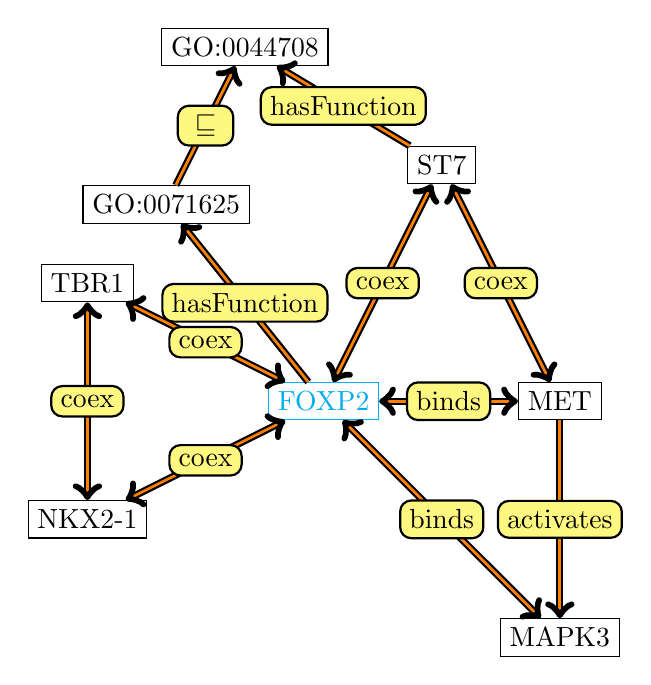
\begin{tikzpicture}
%          \SetUpEdge[lw = 1pt, color = black]
          \GraphInit[vstyle=Shade]
          \tikzset{
            LabelStyle/.style = { rectangle, rounded corners, draw,
              minimum width = 2em, fill = yellow!50,
              text = black },
            VertexStyle/.append style = { inner sep=5pt,
              font = \Large\bfseries},
            EdgeStyle/.append style = {->} }
          
          \SetGraphUnit{5}
          % \tikzset{VertexStyle/.append style={fill}}
          % \tikzset{EdgeStyle/.style={->}}
          \node[draw, color=cyan] (FOXP2) at (0,0) {FOXP2};
          \node[draw] (MET) at (3,0) {MET};
          \node[draw] (ST7) at (1.5,3) {ST7};
          \node[draw] (MAPK3) at (3,-3) {MAPK3};
          \node[draw] (GO0071625) at (-2,2.5) {GO:0071625};
          \node[draw] (GO0044708) at (-1,4.5) {GO:0044708};
          \node[draw] (TBR1) at (-3,1.5) {TBR1};
          \node[draw] (NKX2-1) at (-3,-1.5) {NKX2-1};
          \begin{scope}[/tikz/handle active characters in nodes=false]
          \Edge[label=activates](MET)(MAPK3)
          \Edge[label=hasFunction](FOXP2)(GO0071625)
          \Edge[label=hasFunction](ST7)(GO0044708)
          \Edge[label=$\sqsubseteq$](GO0071625)(GO0044708)

          \tikzset{EdgeStyle/.append style={<->}}
          \Edge[label=binds](FOXP2)(MET)
          \Edge[label=binds](FOXP2)(MAPK3)
          \Edge[label=coex](FOXP2)(TBR1)
          \Edge[label=coex](FOXP2)(NKX2-1)
          \Edge[label=coex](FOXP2)(ST7)
          \Edge[label=coex](MET)(ST7)
          \Edge[label=coex](NKX2-1)(TBR1)
          \end{scope}
          % \tikzset{EdgeStyle/.style={->}}
          % \Edge[label=hf](FOXP2)(GO0044708)
          % \draw[label=binds] (FOXP2) to (MET);
          % \Edge[label=binds](FOXP2)(MET)
          % \Edge[label=activates](MET)(MAPK3)
          % \Edge[label=coexpressed-with](FOXP2)(FOXP4)
          
        \end{tikzpicture}
      }
    \end{column}
    \begin{column}{.4\textwidth}
      \begin{itemize}
      \item precompute the deductive closure:
      \item for all $\phi$: if $\mathcal{KG} \models \phi$, add $\phi$
        to $\mathcal{KG}$
      \end{itemize}
    \end{column}
  \end{columns}
      
\end{frame}

\begin{frame}
  \frametitle{Random walks}
%  \frametitle{Neuro-symbolic feature learning}
  \begin{columns}
    \begin{column}{.6\textwidth}
      \resizebox{1\textwidth}{!}{%
        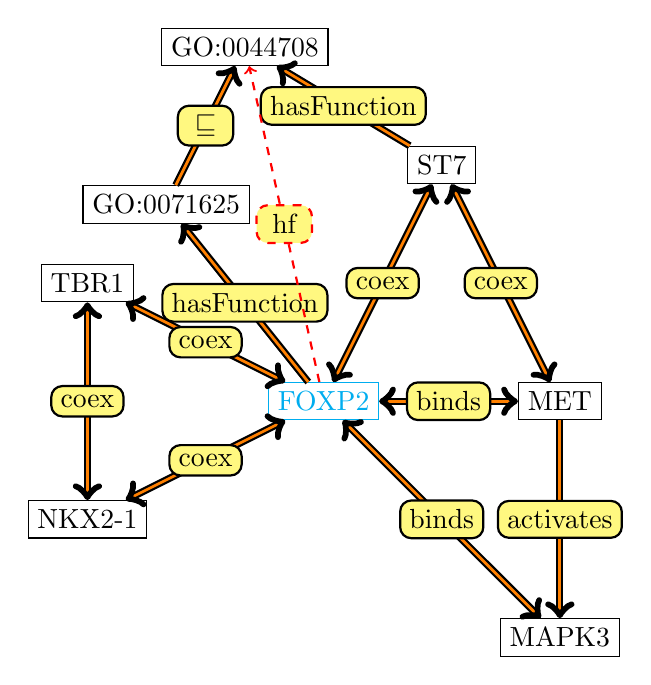
\begin{tikzpicture}
%          \SetUpEdge[lw = 1pt, color = black]
          \GraphInit[vstyle=Shade]
          \tikzset{
            LabelStyle/.style = { rectangle, rounded corners, draw,
              minimum width = 2em, fill = yellow!50,
              text = black },
            VertexStyle/.append style = { inner sep=5pt,
              font = \Large\bfseries},
            EdgeStyle/.append style = {->} }
          
          \SetGraphUnit{5}
          % \tikzset{VertexStyle/.append style={fill}}
          % \tikzset{EdgeStyle/.style={->}}
          \node[draw, color=cyan] (FOXP2) at (0,0) {FOXP2};
          \node[draw] (MET) at (3,0) {MET};
          \node[draw] (ST7) at (1.5,3) {ST7};
          \node[draw] (MAPK3) at (3,-3) {MAPK3};
          \node[draw] (GO0071625) at (-2,2.5) {GO:0071625};
          \node[draw] (GO0044708) at (-1,4.5) {GO:0044708};
          \node[draw] (TBR1) at (-3,1.5) {TBR1};
          \node[draw] (NKX2-1) at (-3,-1.5) {NKX2-1};
          \begin{scope}[/tikz/handle active characters in nodes=false]
          \Edge[label=activates](MET)(MAPK3)
          \Edge[label=hasFunction](FOXP2)(GO0071625)
          \Edge[label=hasFunction](ST7)(GO0044708)
          \Edge[label=$\sqsubseteq$](GO0071625)(GO0044708)

          \tikzset{EdgeStyle/.append style={<->}}
          \Edge[label=binds](FOXP2)(MET)
          \Edge[label=binds](FOXP2)(MAPK3)
          \Edge[label=coex](FOXP2)(TBR1)
          \Edge[label=coex](FOXP2)(NKX2-1)
          \Edge[label=coex](FOXP2)(ST7)
          \Edge[label=coex](MET)(ST7)
          \Edge[label=coex](NKX2-1)(TBR1)

          \tikzset{EdgeStyle/.style={->}}
          \Edge[label=hf, color=red, style=dashed](FOXP2)(GO0044708)
          \end{scope}
          % \tikzset{EdgeStyle/.style={->}}
          % \Edge[label=hf](FOXP2)(GO0044708)
          % \draw[label=binds] (FOXP2) to (MET);
          % \Edge[label=binds](FOXP2)(MET)
          % \Edge[label=activates](MET)(MAPK3)
          % \Edge[label=coexpressed-with](FOXP2)(FOXP4)
          
        \end{tikzpicture}
      }
    \end{column}
    \begin{column}{.4\textwidth}
      \begin{itemize}
      \item precompute the deductive closure:
      \item for all $\phi$: if $\mathcal{KG} \models \phi$, add $\phi$
        to $\mathcal{KG}$
      \end{itemize}
    \end{column}
  \end{columns}
      
\end{frame}


\begin{frame}
  \frametitle{Random walks}
%  \frametitle{Neuro-symbolic feature learning}
  \begin{columns}
    \begin{column}{.6\textwidth}
      \resizebox{1\textwidth}{!}{%
        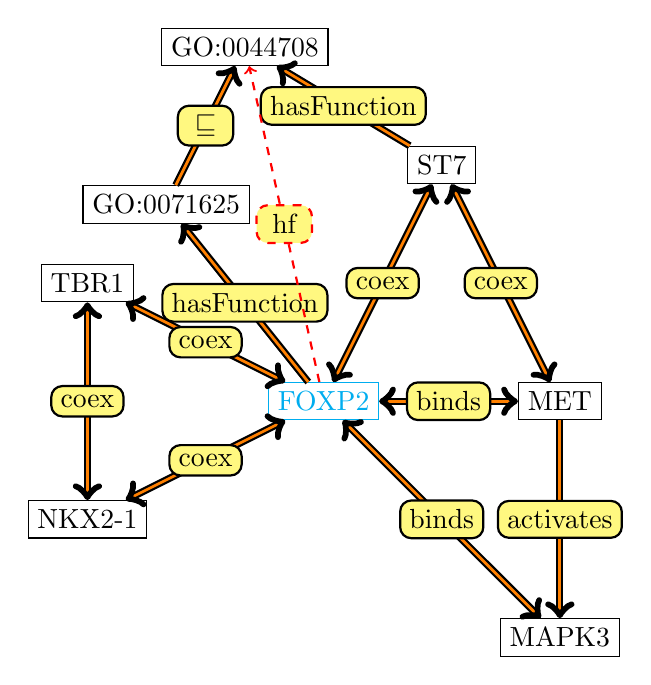
\begin{tikzpicture}
%          \SetUpEdge[lw = 1pt, color = black]
          \GraphInit[vstyle=Shade]
          \tikzset{
            LabelStyle/.style = { rectangle, rounded corners, draw,
              minimum width = 2em, fill = yellow!50,
              text = black },
            VertexStyle/.append style = { inner sep=5pt,
              font = \Large\bfseries},
            EdgeStyle/.append style = {->} }
          
          \SetGraphUnit{5}
          % \tikzset{VertexStyle/.append style={fill}}
          % \tikzset{EdgeStyle/.style={->}}
          \node[draw, color=cyan] (FOXP2) at (0,0) {FOXP2};
          \node[draw] (MET) at (3,0) {MET};
          \node[draw] (ST7) at (1.5,3) {ST7};
          \node[draw] (MAPK3) at (3,-3) {MAPK3};
          \node[draw] (GO0071625) at (-2,2.5) {GO:0071625};
          \node[draw] (GO0044708) at (-1,4.5) {GO:0044708};
          \node[draw] (TBR1) at (-3,1.5) {TBR1};
          \node[draw] (NKX2-1) at (-3,-1.5) {NKX2-1};
          \begin{scope}[/tikz/handle active characters in nodes=false]
          \Edge[label=activates](MET)(MAPK3)
          \Edge[label=hasFunction](FOXP2)(GO0071625)
          \Edge[label=hasFunction](ST7)(GO0044708)
          \Edge[label=$\sqsubseteq$](GO0071625)(GO0044708)

          \tikzset{EdgeStyle/.append style={<->}}
          \Edge[label=binds](FOXP2)(MET)
          \Edge[label=binds](FOXP2)(MAPK3)
          \Edge[label=coex](FOXP2)(TBR1)
          \Edge[label=coex](FOXP2)(NKX2-1)
          \Edge[label=coex](FOXP2)(ST7)
          \Edge[label=coex](MET)(ST7)
          \Edge[label=coex](NKX2-1)(TBR1)

          \tikzset{EdgeStyle/.style={->}}
          \Edge[label=hf, color=red, style=dashed](FOXP2)(GO0044708)
          \end{scope}
          % \draw[label=binds] (FOXP2) to (MET);
          % \Edge[label=binds](FOXP2)(MET)
          % \Edge[label=activates](MET)(MAPK3)
          % \Edge[label=coexpressed-with](FOXP2)(FOXP4)
          
        \end{tikzpicture}
      }
    \end{column}
    \begin{column}{.4\textwidth}
      \begin{itemize}
      \item Exploring the graph:
        \pause
      \item :FOXP2 :binds :MET :coex :ST7 :hasFunction GO:0044708
        \pause
      \item :FOXP2 :hasFunction GO:0071625 subClassOf GO:0044708
        \pause
      \item :FOXP2 :coex :TBR1 :coex :NKX2-1 :coex :TBR1 :coex ...
      \end{itemize}
    \end{column}
  \end{columns}
\end{frame}

\begin{frame}
  \frametitle{Word2Vec}
  Maximize:
  \begin{equation}
    \frac{1}{N} \sum_{n=1}^{N} \sum_{-c\leq j \leq c, j\not=
      0} \log p(w_{n+j}|w_n)
  \end{equation}
  with
  \begin{equation}
    p(w_o | w_i) = \frac{\exp({v'_{w_o}}^T v_{w_i})}{\sum_{w=1}^{W}
      \exp({v'_{w}}^T v_{w_i})}
  \end{equation}
  (at least conceptually; different strategies are used to approximate Eqn. 2)
\end{frame}

\begin{frame}
  \frametitle{Word2Vec and Random Walks}
  \begin{itemize}
  \item random walks ``flatten'' a graph
    \begin{itemize}
    \item walks capture node neighborhood
    \item and generate a ``corpus''
    \end{itemize}
  \item random walks capture graph ``structure''
    \begin{itemize}
    \item hub-nodes, communities, etc.
    \item determine ``importance'' of nodes
    \end{itemize}
  \item embeddings capture co-occurrence
    \begin{itemize}
    \item similar graph neighborhood $\Rightarrow$ similar
      co-occurrence $\Rightarrow$ similar vector
    \end{itemize}
  \item embeddings generate ``feature'' vectors
    \begin{itemize}
    \item functions from symbols (words, labels) into $\Re^n$
    \end{itemize}
  \end{itemize}
\end{frame}

\begin{frame}
  \frametitle{What to do with embeddings?}
  \begin{itemize}
  \item useful for edge prediction, similarity, clustering, as feature
    vectors
    \begin{itemize}
    \item supervised: edge prediction (e.g., SVM, ANN)
      \begin{itemize}
      \item e.g.: find a function $f:\Re^n \times \Re^n \mapsto [0,1]$
        s.t. $\sqrt \frac{\sum_{t=1}^T (\hat{y_t} - y_t)^2}{T}$ (RMSE)
        is minimized for a set of true labels $y_k$
      \end{itemize}
    \item unsupervised: clustering, similarity, visualization
      \begin{itemize}
      \item cosine similarity (for L2-normalized features)
      \item Word2Vec embeddings capture similarity between co-occurrence vectors
      \end{itemize}
    \end{itemize}
  \end{itemize}
\end{frame}

\begin{frame}
  \frametitle{Visualizing embeddings}
%  \frametitle{Neuro-symbolic feature learning}
  \centerline{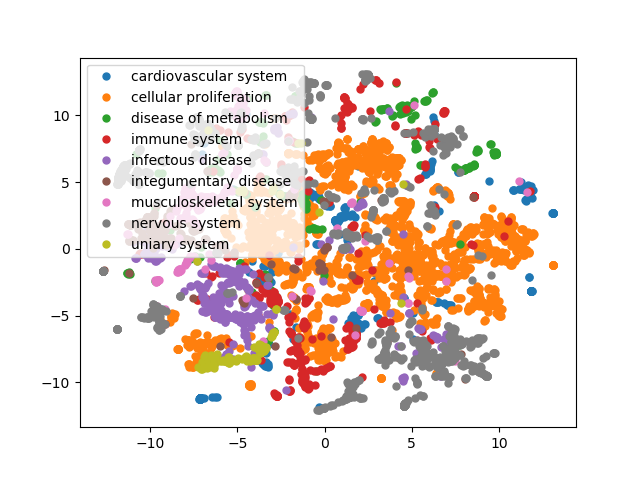
\includegraphics[width=\textwidth]{graph-tsne.png}}
\end{frame}

\begin{frame}
  \frametitle{Supervised learning}
  \begin{itemize}
  \item feature vectors represent graph neighborhood of nodes
    \begin{itemize}
    \item adjacent nodes and edges
    \item ontology classes (asserted \& inferred)
    \end{itemize}
  \item useful in supervised prediction tasks
  \item relation prediction:
    \begin{itemize}
    \item input: two features vectors (from embedding function)
    \item output: $0$ or $1$ (relation or not)
    \item training data: positive and negative cases
      \begin{itemize}
      \item $R(x,y)$ and $\neg R(x,y)$
      \end{itemize}
    \end{itemize}
  \end{itemize}
\end{frame}

\begin{frame}
  \frametitle{Features: supervised learning}
  \resizebox{\textwidth}{!}{
  \begin{tabular}{@{}lllcccc@{}}\toprule 
      \multirow{2}{*}{Object property} 
      & Source type & Target type &\multicolumn{2}{c}{Without reasoning}&\multicolumn{2}{c}{With reasoning}\\
      &&& F-measure & AUC & F-measure & AUC \\
      \midrule
      has target & Drug & Gene/Protein & 0.94 & 0.97 & 0.94 & 0.98 \\
      has disease annotation & Gene/Protein & Disease & 0.89 & 0.95 & 0.89 & 0.95 \\
      has side-effect$^*$ & Drug & Phenotype & 0.86 & 0.93 & 0.87 & 0.94 \\
      has interaction & Gene/Protein & Gene/Protein & 0.82 & 0.88 & 0.82 & 0.88\\
      has function$^*$ & Gene/Protein & Function & 0.85 & 0.95 & 0.83 & 0.91 \\
      has gene phenotype$^*$  & Gene/Protein & Phenotype & 0.84 & 0.91 & 0.82 & 0.90  \\
      has indication & Drug & Disease & 0.72 & 0.79 & 0.76 & 0.83 \\
      has disease phenotype$^*$  & Disease & Phenotype & 0.72 & 0.78 & 0.70 & 0.77 \\
    \end{tabular}}
\end{frame}

\begin{frame}
  \frametitle{Some limitations}
  \begin{itemize}
  \item ``word''-based (Word2Vec):
    \begin{itemize}
    \item semantics is reduced to co-occurrence (in ABox/TBox
      statements)
    \item ``disjointWith'' vs. ``part-of'' vs. ``subClassOf''
    \end{itemize}
  % \item graph-based:
  %   \begin{itemize}
  %   \item ontologies are not graphs!
  %   \item converting ontologies to graphs loses information
  %   \item no axioms, no definitions
  %   \end{itemize}
  \end{itemize}
\end{frame}



\end{document}
%%% Local Variables:
%%% mode: latex
%%% TeX-master: t
%%% End:
